\section{ハミルトニアンの基底変換}
ここでは、Hamiltonianの基底変換を行う。
\begin{eqnarray}
    \hat{\mathcal{H}}&=&\hbar\biggl(\hat{a}^{\dagger }\ \hat{b}^{\dagger }\biggr)\biggl(\begin{array}{cc}
    \tilde{\omega}_{a} & g_{eff}(\Phi ) \\
    g_{eff}(\Phi ) & \tilde{\omega}_{b}
    \end{array}\biggr)\biggl(\begin{array}{l}
    \hat{a} \\
    \hat{b}
    \end{array}\biggr)\\ \\
    &=& \hbar \tilde{\omega}_{a} \hat{a}^{\dagger} \hat{a}+\hbar \tilde{\omega}_{b} \hat{b}^{\dagger} \hat{b}+\hbar g_{eff}(\Phi)\biggl(\hat{a}^{\dagger}\hat{b}+ \hat{b}^{\dagger}\hat{a}\biggr)
\end{eqnarray}
ここで共振器A,Bのそれぞれの生成消滅演算子$\hat{a}{\dagger},\hat{a},\hat{b}{\dagger},\hat{b},$を結合モードの生成消滅演算子$\hat{c}_{+}^{\dagger},\hat{c}_{+},\hat{c}_{-}^{\dagger},\hat{c}_{-}$で変換する。
%演算子
\begin{equation}
    \hat{c}_{\pm}=\frac{\hat{a} \pm \hat{b}}{\sqrt{2}} ,\quad \hat{c}_{\pm}^{\dagger}=\frac{\hat{a}^{\dagger} \pm \hat{b}^{\dagger}}{\sqrt{2}}
\end{equation}
結合モードの生成消滅で元の演算子を書き表すと
\begin{equation}
    \hat{a}=\frac{\hat{c}_{+}+\hat{c}_{-}}{\sqrt{2}} ,\quad \hat{b}=\frac{\hat{c}_{+}-\hat{c}_{-}}{\sqrt{2}}
\end{equation}
\begin{equation}
    \hat{a}^{\dagger}=\frac{\hat{c}_{+}^{\dagger}+\hat{c}_{-}^{\dagger}}{\sqrt{2}} ,\quad \hat{b}^{\dagger}=\frac{\hat{c}_{+}^{\dagger}-\hat{c}_{-}^{\dagger}}{\sqrt{2}}
\end{equation}
となる。よってその演算子の積は
%積
\begin{equation}
    \hat{a}^{\dagger} \hat{a}=\frac{1}{2}\biggl(\hat{c}_{+}^{\dagger}+\hat{c}_{-}^{\dagger}\biggr) \biggl(\hat{c}_{+}+\hat{c}_{-}\biggr) ,\quad \hat{a}^{\dagger} \hat{b}=\frac{1}{2}\biggl(\hat{c}_{+}^{\dagger}+\hat{c}_{-}^{\dagger}\biggr)\biggl(\hat{c}_{+}-\hat{c}_{-}\biggr)
\end{equation}
\begin{equation}
    \hat{b}^{\dagger} \hat{b}=\frac{1}{2}\biggl(\hat{c}_{+}^{\dagger}-\hat{c}_{-}^{\dagger}\biggr)\biggl(\hat{c}_{+}-\hat{c}_{-}\biggr) ,\quad \hat{b}^{\dagger}\hat{a} = \frac{1}{2}\biggl(\hat{c}_{+}^{\dagger}-\hat{c}_{-}^{\dagger}\biggr)\biggl(\hat{c}_{+}+\hat{c}_{-}\biggr)
\end{equation}
と表現できる。それぞれ計算を進めると

\begin{equation}
    \hat{a}^{\dagger} \hat{a}=\frac{1}{2}\biggl(\hat{c}_{+}^{\dagger} \hat{c}_{+}+\hat{c}_{+}^{\dagger} \hat{c}_{-}+\hat{c}_{-}^{\dagger} \hat{c}_{+}+\hat{c}_{-}^{\dagger} \hat{c}_{-}\biggr)
\end{equation}
\begin{equation}
    \hat{b}^{\dagger} \hat{b}=\frac{1}{2}\biggl(\hat{c}_{+}^{\dagger} \hat{c}_{+}-\hat{c}_{+}^{\dagger} \hat{c}_{-}-\hat{c}_{-}^{\dagger} \hat{c}_{+}+\hat{c}_{-}^{\dagger} \hat{c}_{-}\biggr)
\end{equation}

\begin{equation}
    \hat{a}^{\dagger} \hat{b}=\frac{1}{2}\biggl(\hat{c}_{+}^{\dagger}\hat{c}_{+}-\hat{c}_{+}^{\dagger} \hat{c}_{-}+\hat{c}_{-}^{\dagger} \hat{c}_{+}-\hat{c}_{-}^{\dagger} \hat{c}_{-}\biggr)
\end{equation}
\begin{equation}
    \hat{b}^{\dagger}\hat{a} =\frac{1}{2}\biggl(\hat{c}_{+}^{\dagger}\hat{c}_{+} +\hat{c}_{+}^{\dagger}\hat{c}_{-} - \hat{c}_{-}^{\dagger}\hat{c}_{+}-\hat{c}_{-}^{\dagger}\hat{c}_{-}\biggr)
\end{equation}

これを元のハミルトニアンに代入すれば

\begin{equation}
    \hat{H}=\frac{\hbar}{2} \hat{\omega}_{a}\biggl(\hat{c}_{+}^{\dagger} \hat{c}_{+}+\hat{c}_{+}^{\dagger} \hat{c}_{-}+\hat{c}_{-}^{\dagger} \hat{c}_{+}+\hat{c}_{-}^{\dagger} \hat{c}_{-}\biggr)+\frac{\hbar}{2} \hat{\omega}_{b}\biggl(\hat{c}_{+}^{\dagger} \hat{c}_{+}-\hat{c}_{+}^{\dagger} \hat{c}_{-}-\hat{c}_{-}^{\dagger} \hat{c}_{+}+\hat{c}_{-}^{\dagger} \hat{c}_{-}\biggr)
\end{equation}
\begin{equation}
    +\frac{\hbar}{2} g_{eff}\biggl(\hat{c}_{+}^{\dagger}\hat{c}_{+}-\cancel{\hat{c}_{+}^{\dagger} \hat{c}_{-}}+\bcancel{\hat{c}_{-}^{\dagger} \hat{c}_{+}}-\hat{c}_{-}^{\dagger} \hat{c}_{-}+\hat{c}_{+}^{\dagger}\hat{c}_{+} +\cancel{\hat{c}_{+}^{\dagger}\hat{c}_{-}} - \bcancel{\hat{c}_{-}^{\dagger}\hat{c}_{+}}-\hat{c}_{-}^{\dagger}\hat{c}_{-}\biggr)
\end{equation}

式を整理すると

\begin{equation}
    \hat{H}=\frac{\hbar}{2}\biggl(\hat{\omega}_{a}+\hat{\omega}_{b}+2 g(\Phi)\biggr) \hat{c}_{+}^{\dagger} \hat{c}_{+}+\frac{\hbar}{2}\biggl(\hat{\omega} a+\hat{\omega}_{b}-2 g(\Phi)\biggr) \hat{c}_{-}^{\dagger} \hat{c}_{-}
\end{equation}
\begin{equation}
    +\frac{\hbar}{2}\biggl(\hat{\omega}_{a}-\hat{\omega}_{b}\biggr)\biggl(\hat{c}_{+}^{\dagger}\hat{c}_{-}-\hat{c}_{-}^{\dagger} \hat{c}_{+}\biggr)
\end{equation}
ここで第1項と第2項を
\begin{equation}
    \Omega_{+}=\frac{\tilde{\omega}_{a}+\tilde{\omega}_{b}}{2} + g_{eff}(\Phi)
\end{equation}
\begin{equation}
    \Omega_{-}=\frac{\tilde{\omega}_{a}+\tilde{\omega}_{b}}{2} - g_{eff}(\Phi)
\end{equation}
第3項を
\begin{equation}
    \Delta = \frac{\tilde{\omega}_{a}-\tilde{\omega}_{b}}{2}
\end{equation}
とすれば元のハミルトニアンは
\begin{eqnarray}
    \hat{H}&=&\hbar\Omega_{+} \hat{c}_{+}^{\dagger} \hat{c}_{+}+\hbar\Omega_{-} \hat{c}_{-}^{\dagger} \hat{c}_{-} +\hbar \Delta \biggl(\hat{c}_{+}^{\dagger}\hat{c}_{-}-\hat{c}_{-}^{\dagger} \hat{c}_{+}\biggr)\\ \\ 
    &=& \hbar\biggl(\begin{array}{cc}
        \hat{c}_{+}^{\dagger} & \hat{c}_{-}^{\dagger}
        \end{array}\biggr)\biggl(\begin{array}{cc}
        \Omega_{+} & \Delta \\
        \Delta & \Omega_{-}
        \end{array}\biggr)\biggl(\begin{array}{l}
        \hat{c}_{+} \\
        \hat{c}_{-}
        \end{array}\biggr)
\end{eqnarray}

のように結合モードの基底で書き表すことができる。

\section{rf-SQUIDの相互インダクタンス}
dc-SQUIDのインダクタンスは
\begin{equation}
    L_{s}(\Phi)=\frac{\Phi_0}{4\pi I_{c}|{\cos({\phi_{-}^{min}(\Phi_{ext})}})|}
\end{equation}
と記述することができる。
\begin{equation}
    \Phi=\Phi_{ext}+L_{loop}
\end{equation}
\begin{equation}
    \beta_{dc}=\frac{2\pi L_{loop} I_{c}}{\Phi_{0}}
\end{equation}
とすると。
\section{インターデジタルキャパシタンス}
インターデジタルキャパシタンスとは図中の共振器の櫛状になっている部分の構造である。
\begin{figure}[H]
    \label{le}
    \centering
    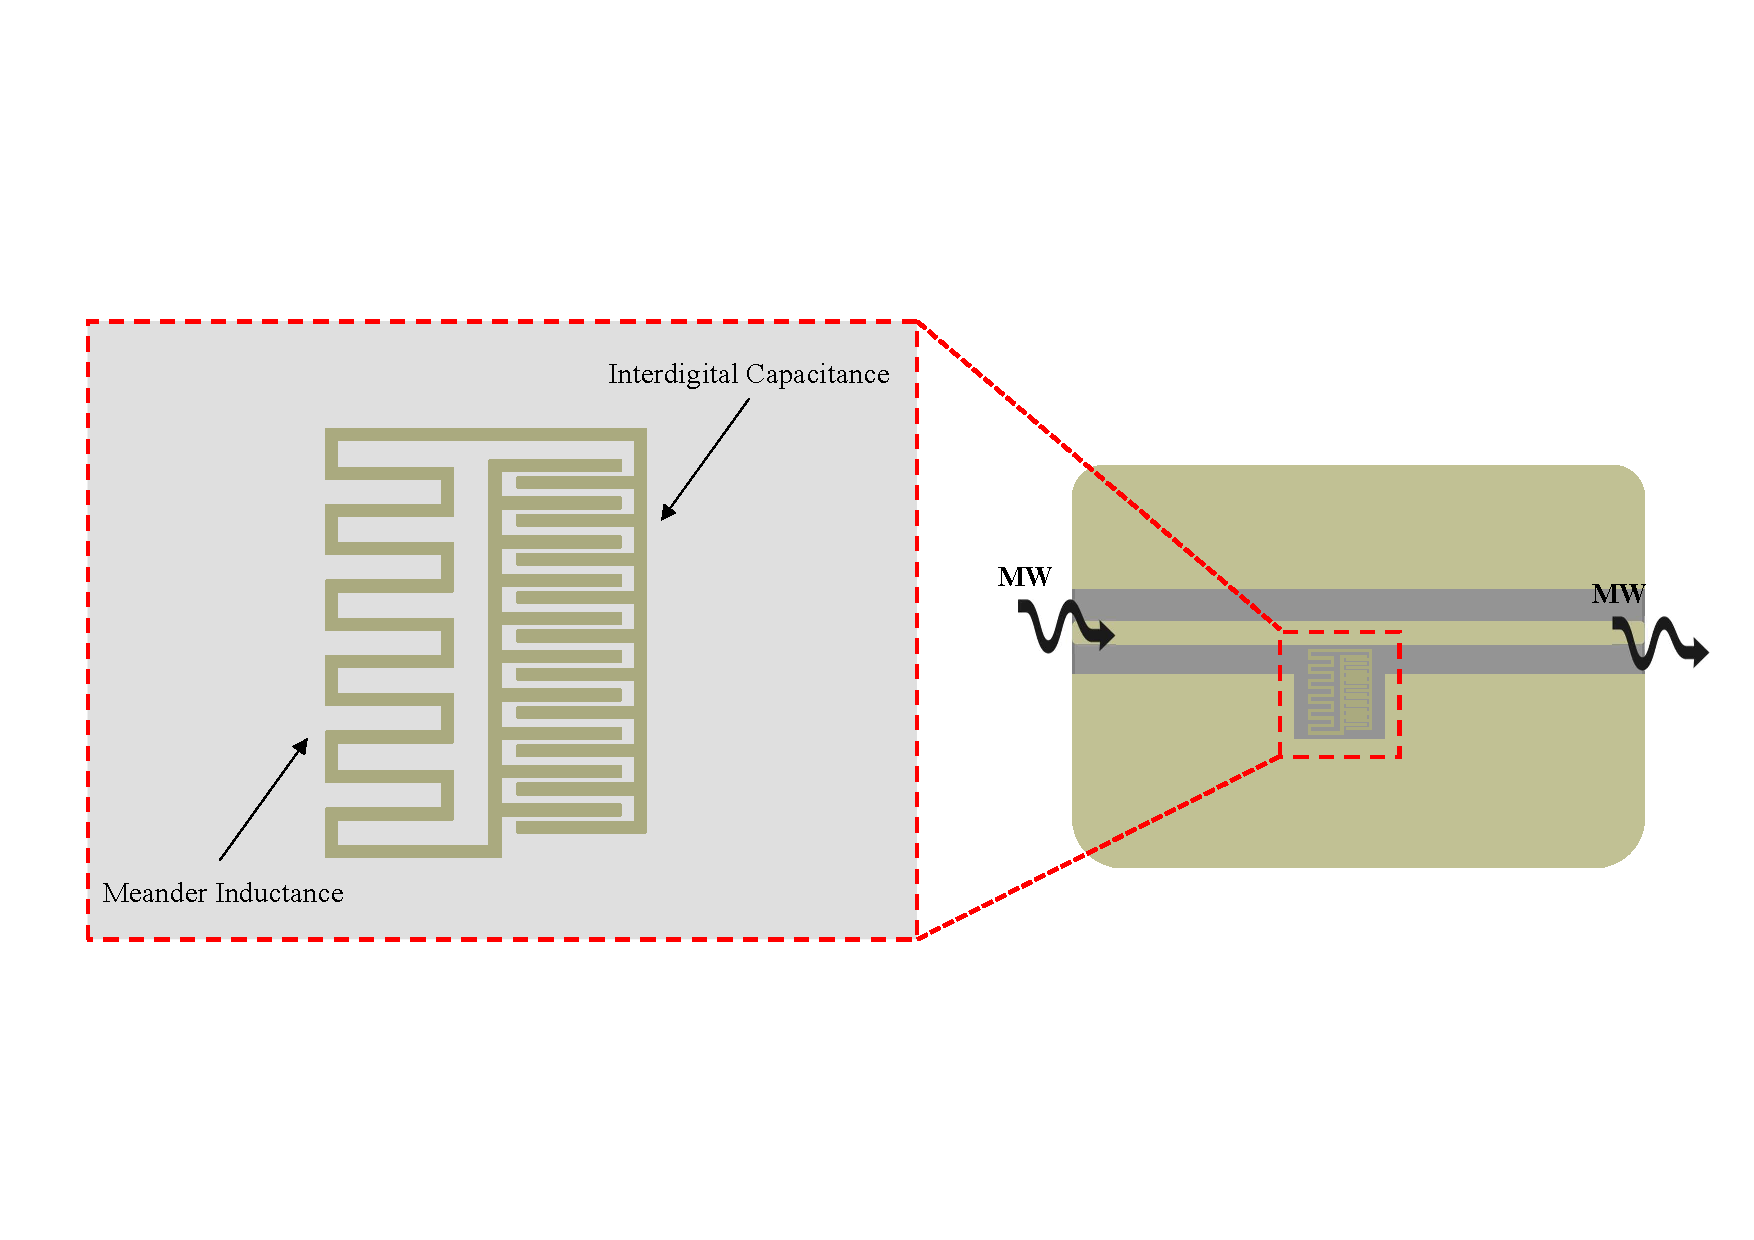
\includegraphics[width=16cm]{lumpedelement.pdf}
    \caption{準集中定数型共振器(再掲)}
\end{figure}
この構造により、電極同士の表面積を上げることでキャパシタンスを増幅することができる。ここではインターデジタルキャパシタンスの計算方法について解説を行う。また、ここで解説するインターデジタルキャパシタンスの計算方法は櫛の数が2本以上のケースである。\cite*{Gevorgian1996,Dib2005,Dib2001ComprehensiveSO}
\begin{figure}[H]
    \centering
    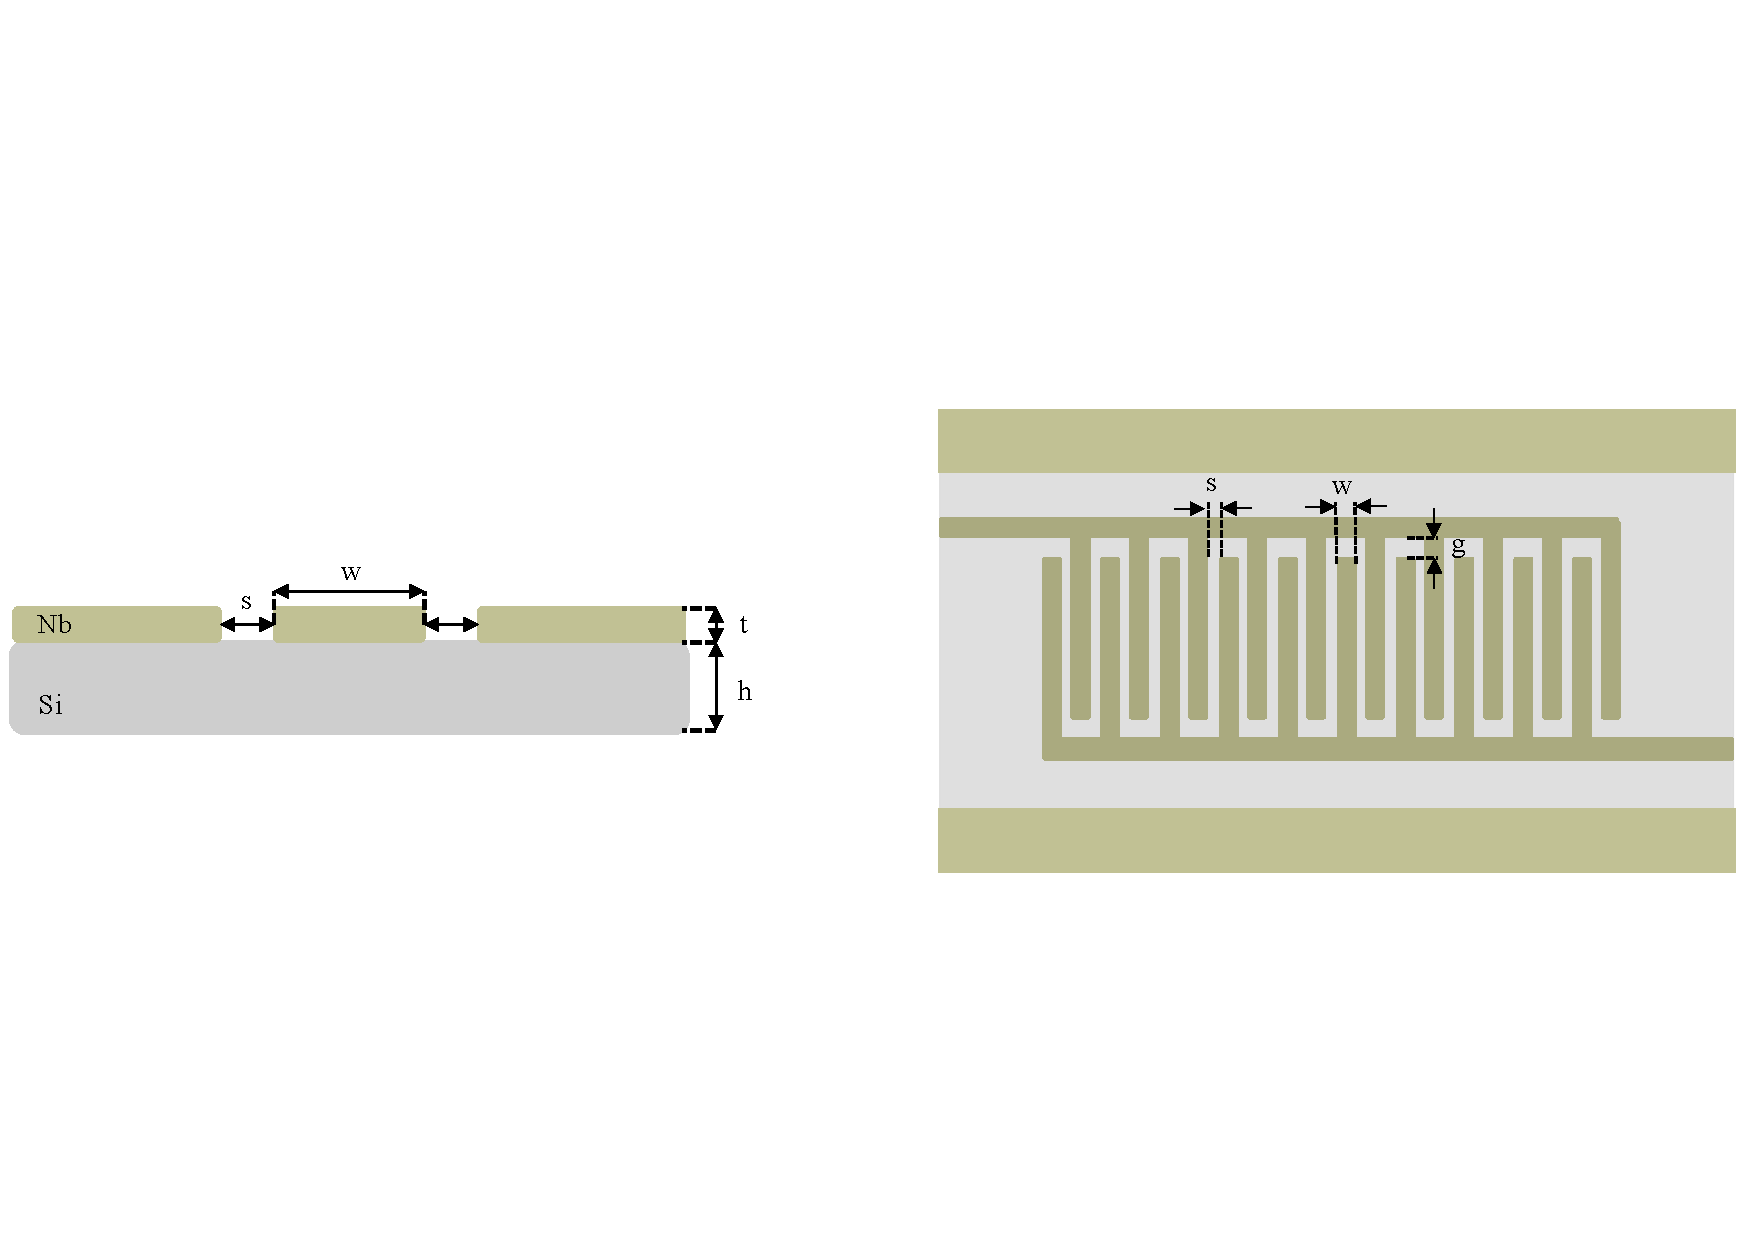
\includegraphics[width=14cm]{IDC2.pdf}
    \caption{インターデジタルキャパシタンス}
\end{figure}
式中の文字は上記の図中のパラメータに対応している。
まず線路の幅wは導体の厚さを含めた実行幅$w_eff$へと変換を行う。\cite*{Gevorgian1996}
\begin{equation}
    W_{e f f}=W+\frac{t}{\pi}\biggl(1+\ln \biggl(\frac{4 \pi W}{t}\biggr)\biggr)
\end{equation}
ここで相対する導体間のキャパシタンスをCsとする。
キャパシタンスCsを構成するのは櫛が3本であることを想定したキャパシタンスC3、櫛の本数Nに相当するキャパシタンス開放状態になっている最両端の櫛のキャパシタンスCendの3つである。
\begin{equation}
    C_{s}=C_{3}+C_{N}+C_{\text { end }}
\end{equation}
それぞれのキャパシタンスはコンフォーマルマッピングを用いて解析的に求めることが可能である。それぞれの値を求めるにはまずC3について
\begin{equation}
    C_{3}=4 \varepsilon_{0} \varepsilon_{e} \frac{K\biggl(k_{1}\biggr)}{K\biggl(k_{1}^{\prime}\biggr)} L
\end{equation}\begin{equation}
    \varepsilon_{e}=1+q_{1} \frac{\varepsilon_{r}-1}{2}
\end{equation}
\begin{equation}
        q_{1}=\frac{K\biggl(k_{1}^{\prime}\biggr)}{K\biggl(k_{1}\biggr)} \frac{K\biggl(k_{2}\biggr)}{K\biggl(k_{2}^{\prime}\biggr)}
\end{equation}
\begin{equation}
    k_{1}=\frac{W}{W+2 S} \sqrt{\frac{1-\biggl(\frac{W+2 S}{3 W+2 S}\biggr)^{2}}{1-\biggl(\frac{W}{3 W+2 S}\biggr)^{2}}}
\end{equation}
\begin{equation}
    \begin{aligned}
    k_{2}=& \frac{\sinh \biggl(\frac{\pi W}{4 h}\biggr)}{\sinh \biggl(\frac{\pi(W+2 S)}{4 h}\biggr)} 
    & \sqrt{\frac{\sinh ^{2}\biggl(\frac{\pi(3 W+2 S)}{4 h}\biggr)-\sinh ^{2}\biggl(\frac{\pi(W+2 S)}{4 h}\biggr)}{\sinh ^{2}\biggl(\frac{\pi(3 W+2 S)}{4 h}\biggr)-\sinh ^{2}\biggl(\frac{\pi W}{4 h}\biggr)}}
    \end{aligned}
\end{equation}
同様にしてCNについて求めると
\begin{equation}
    C_{N}=(N-3) \varepsilon_{0} \varepsilon_{N} \frac{K\biggl(k_{3}\biggr)}{K\biggl(k_{3}^{\prime}\biggr)} L
\end{equation}
\begin{equation}
    \varepsilon_{N}=1+q_{N} \frac{\varepsilon_{r}-1}{2}
\end{equation}
\begin{equation}
    q_{N}=\frac{K\biggl(k_{3}^{\prime}\biggr)}{K\biggl(k_{3}\biggr)} \frac{K\biggl(k_{4}\biggr)}{K\biggl(k_{4}^{\prime}\biggr)},
\end{equation}
\begin{equation}
    k_{3}=\frac{W}{W+S},
\end{equation}
\begin{equation}
    \begin{aligned}
    k_{4}=& \frac{\sinh \biggl(\frac{\pi W}{4 h}\biggr)}{\sinh \biggl(\frac{\pi(W+ S)}{4 h}\biggr)} 
    & \sqrt{\frac{\sinh ^{2}\biggl(\frac{\pi(W+S)}{4 h}\biggr)+\sinh ^{2}\biggl(\frac{\pi(W+ S)}{4 h}\biggr)}{\cosh ^{2}\biggl(\frac{\pi(W)}{4 h}\biggr)-\sinh ^{2}\biggl(\frac{\pi (W+S)}{4 h}biggrt)}}
    \end{aligned}
\end{equation}
として求まる。最後にCendについて、この計算を行う上で主に参考にしている論文\cite*{Dib2005}ではCendの計算について\cite*{Dib2001ComprehensiveSO}中の式
\begin{equation}
    C_{o c}=c_{e f f} C_{o e}\biggl(\epsilon_{r}=1\biggr)
\end{equation}
\begin{equation}
    \label{Cend}
    C_{\alpha c}\biggl(c_{r}=1\biggr)=\frac{c_{0}}{\pi}\biggl(\frac{1}{g^{2}} f_{s}(g, W+S, 0)+\frac{1}{W^{2}} f_{0}(W, S, 0)\biggr)
\end{equation}
\begin{equation}
    \label{fs}
    \begin{aligned}
    f_{s}(a, b, c) &=\frac{4}{3} c^{3}+f(a, c)+f(b, c)-4 a b c \tan ^{-1}\biggl(\frac{a b}{c \tau}\biggr)-\frac{2}{3}\biggl(b^{2}-2 c^{2}+a^{2}\biggr) \tau \\
    &+\biggl(a^{2}-c^{2}\biggr) b \ln \biggl(\frac{\tau+b}{\tau-b}\biggr)+\biggl(b^{2}-c^{2}\biggr) a \ln \biggl(\frac{\tau+a}{\tau-a}\biggr)
    \end{aligned}
\end{equation}
\begin{equation}
    \label{f0}
    f_{0}(a, b, c) =\frac{4}{3} c^{3}+f(a, c)+f(a+b, c)-\frac{1}{2} f(b+2 a, c)-\frac{1}{2} f(b, c)
\end{equation}
\begin{equation}
    \label{fx}
    f(x, y) =\frac{2}{3}\biggl(x^{2}-2 y^{2}\biggr) \sqrt{x^{2}+y^{2}}+y^{2} x \ln \biggl(\frac{\sqrt{x^{2}+y^{2}}+x}{\sqrt{x^{2}+y^{2}}-x}\biggr)
\end{equation}
を使用したと記述されているが式\ref*{fx}の第2項目は不適切であるため、本稿では含めずに計算した。というのも式\ref*{fx}が使用されている式\ref{Cend,fs,f0}に注目すると式\label{fx}中の$y$は常にゼロであり、第2項目は2乗でゼロに収束する。よって2項目は計算に含まれないことになる。よって計算には以下
\begin{equation}
    \label{fx_re}
    f(x, y)_{revised} =\frac{2}{3}\biggl(x^{2}-2 y^{2}\biggr) \sqrt{x^{2}+y^{2}}
\end{equation}
をもちいた。
以上の計算式を用いてインターデジタルキャパシタンスの値を見積もることができる。
ここではさらに本稿で使用したパラメータを用いて櫛の本数Nに対してキャパシタンスの値がどれだけ変化するのか、また、実験結果との比較を行う。
\begin{figure}[H]
    \centering
    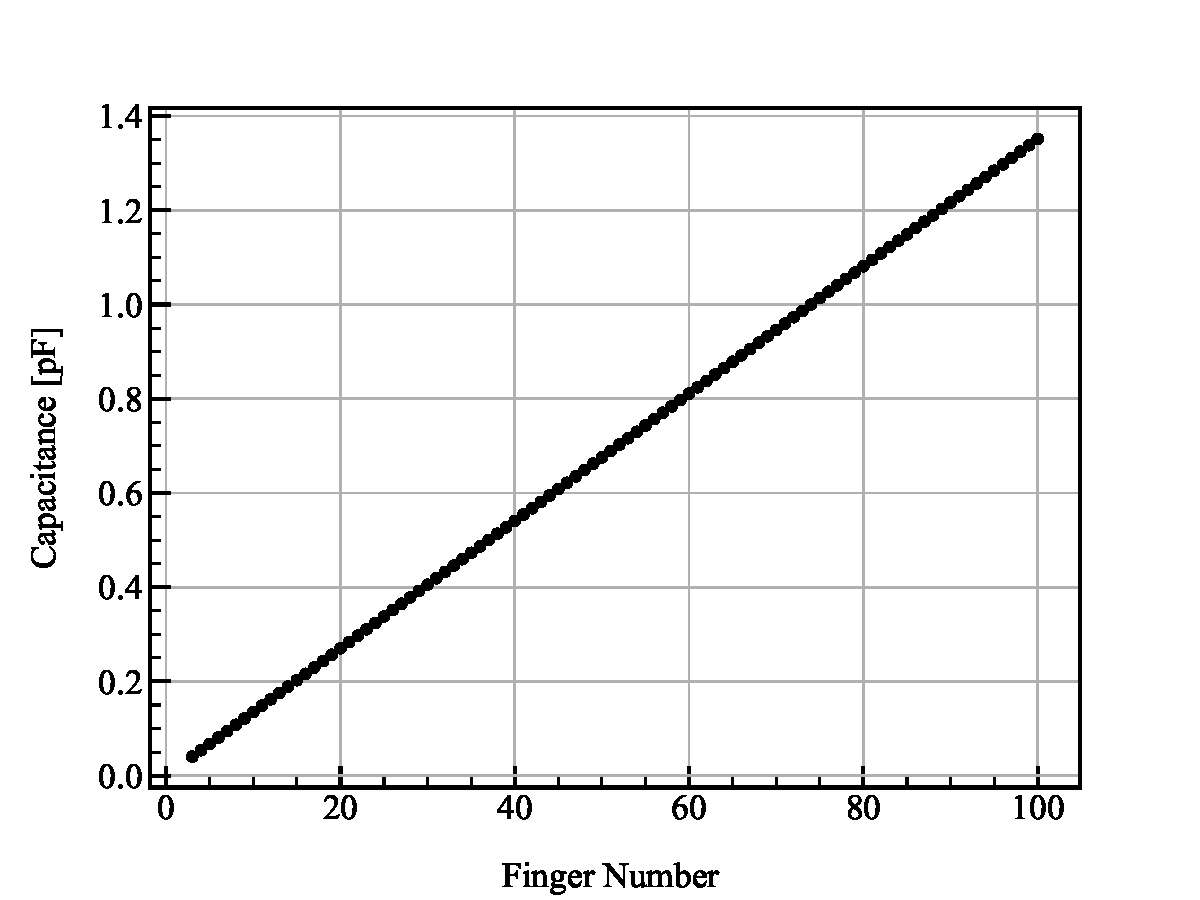
\includegraphics[width=10cm]{IDC_cal.pdf}
    \caption{キャパシタンス vs 櫛の本数}
\end{figure}
\section{ミアンダインダクタンス}
ミアンダインダクタンスとは図\ref{le}中蛇行した構造を持ったインダクタのことを指している。蛇行させることによりサイズに対して線路長が長くなり、また、相対する相互インダクタンスによりインダクタンスの総和が増加する。ここでは本稿で用いたミアンダインダクタンスの解析的計算方法について解説する。本文中ではここで行った解析的計算の結果と電磁界シミュレーションによるミアンダインダクタンス部分の計算を比較していので参照されたい。
\begin{figure}[H]
    \label{ミアンダ}
    \centering
    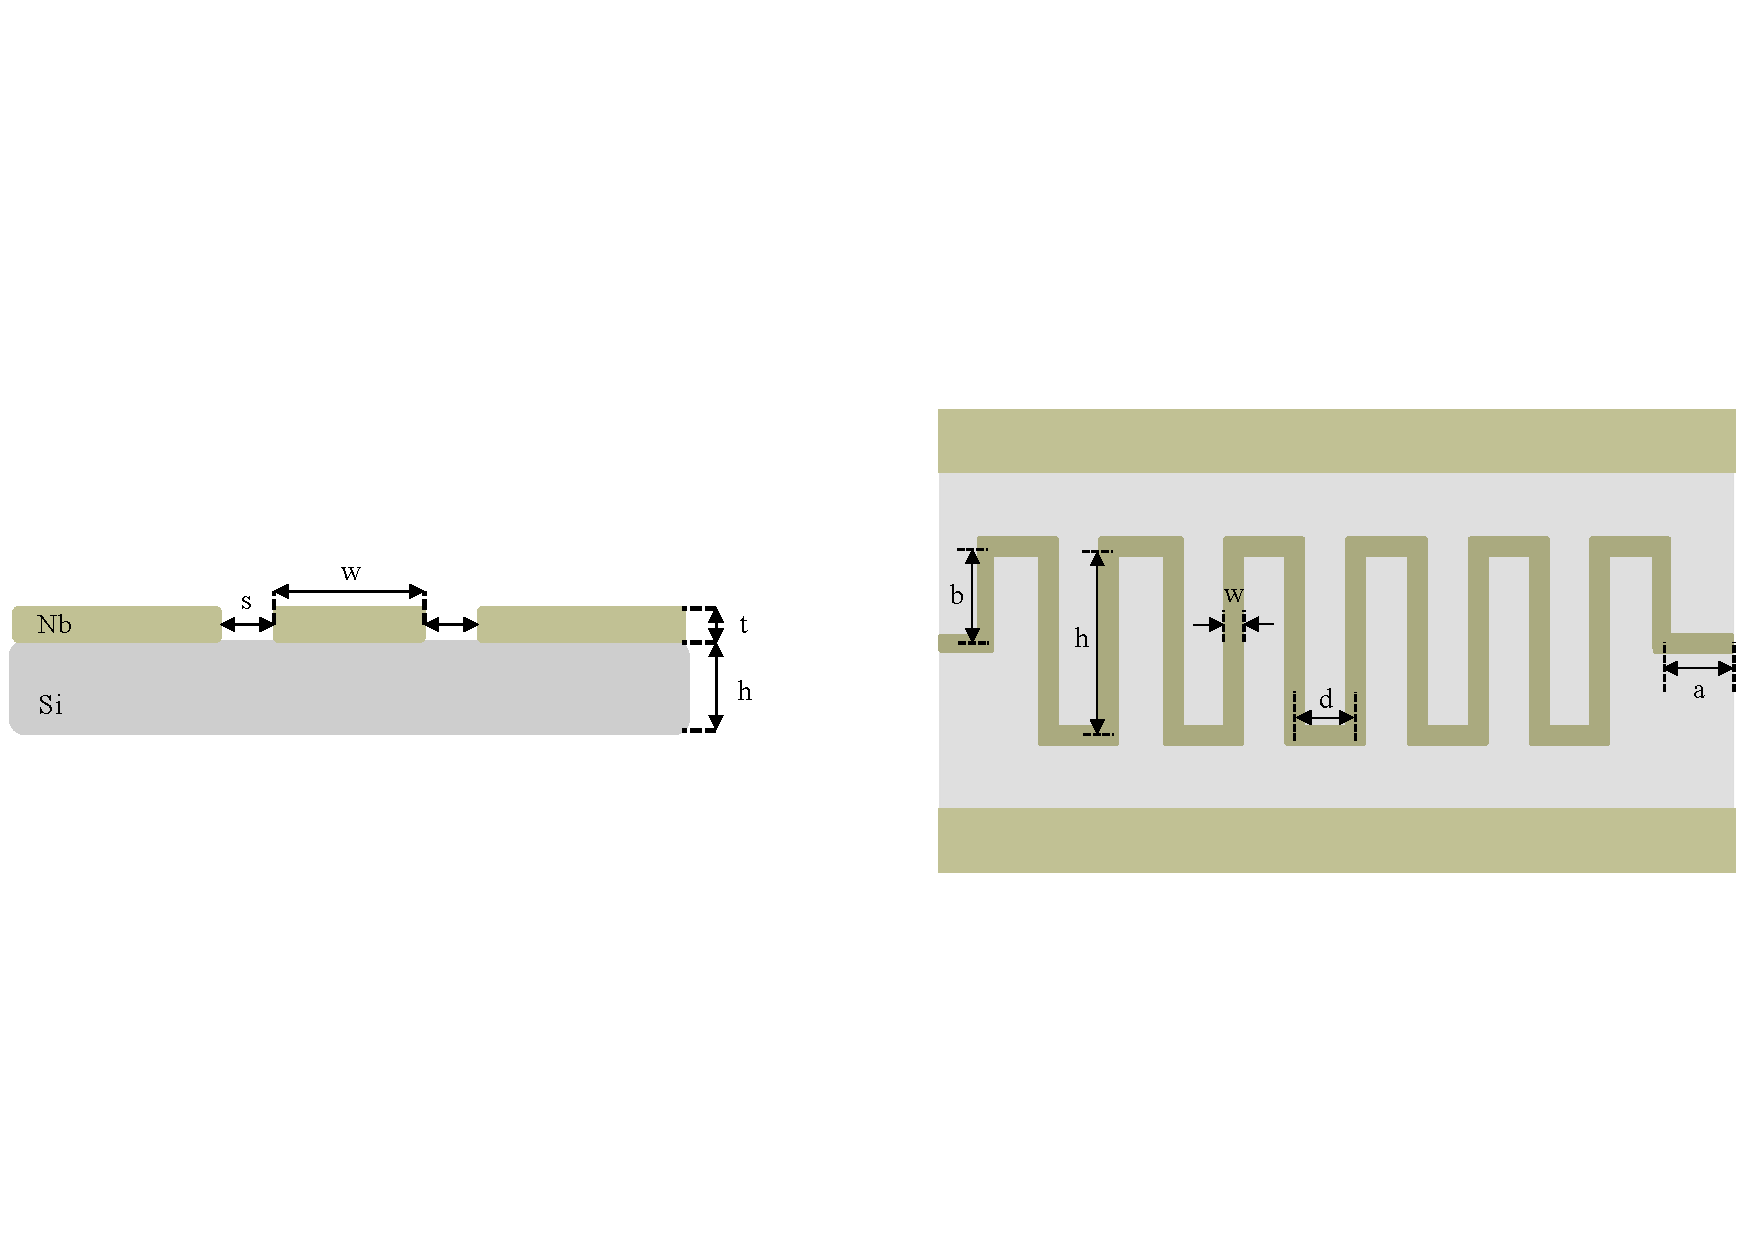
\includegraphics[width=14cm]{ミアンダ.pdf}
    \caption{ミアンダインダクタンス}
\end{figure}
以下数式は上図のパラメータに対応する。この計算に主に参考にした論文は\cite*{Stojanovic2004}である。
文献\cite*{Grover}より長方形線路の自己インダクタンスは
\begin{equation}
    L=0.002 l\{\ln [2 l /(w+t)]+0.50049+[(w+t) / 3 l]\}
\end{equation}
である。ここでwは線路幅、tは厚さ、lは線路長である。ミアンダインダクタンスの大部分を占めているのは各セグメントに於ける自己インダクタンスの総和である。すなわち、図中のパラメータによって各セグメントをラベル付けするとミアンダインダクタンス中セルフインダクタンスの寄与は
\begin{equation}
    L_{\text {selftot }}=2 \cdot L_{a}+2 \cdot L_{b}+N \cdot L_{h}+(N+1) \cdot L_{d}
\end{equation}
である。ここでNはセグメントhの本数に対応する。図\ref*{ミアンダ}ではN=10である。参考文献ではいくつかタイプミスが見受けられたため、少々煩雑ではあるが式の全文を記すこととする。
既に記した条件を前提とした上でNがの偶奇で計算は異なる。
\begin{figure}[H]
    \label{偶奇}
    \centering
    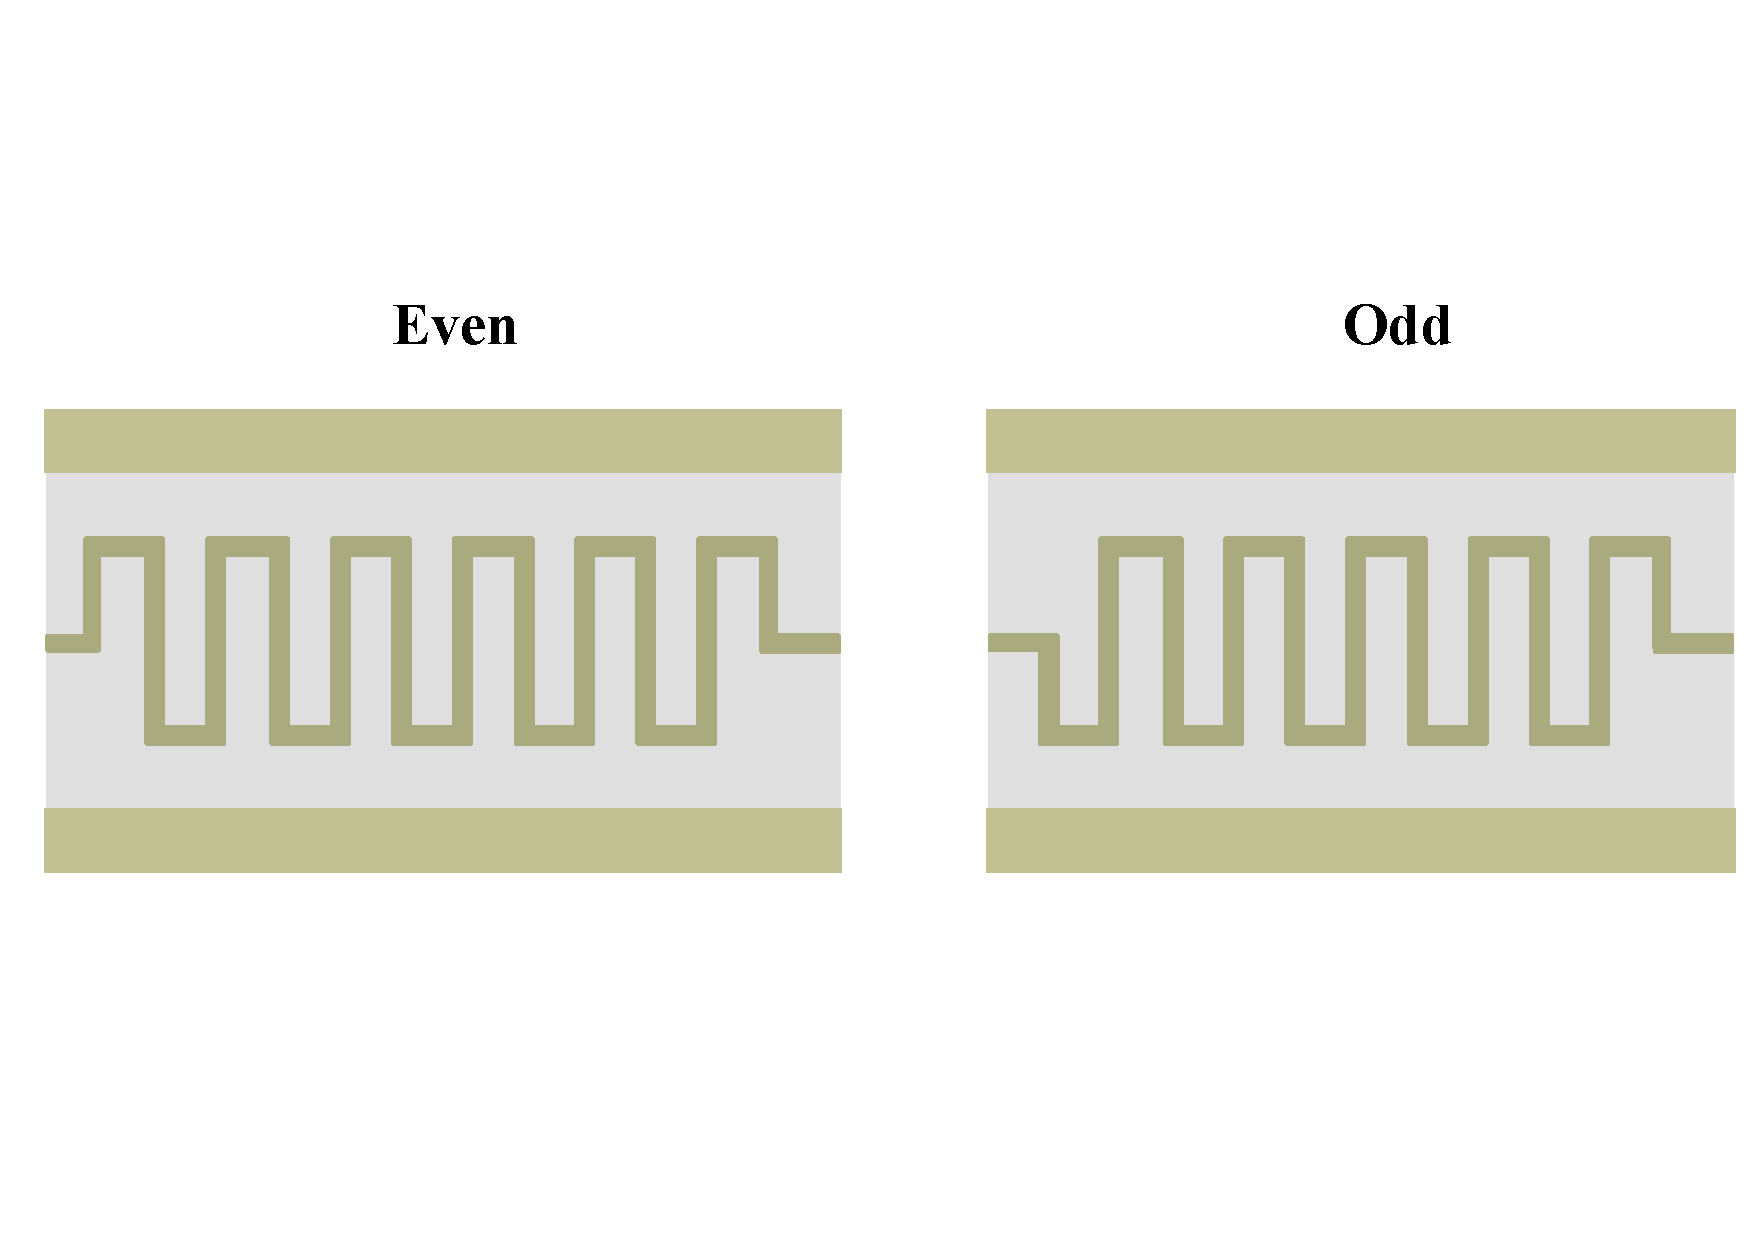
\includegraphics[width=14cm]{偶奇.pdf}
    \caption{ミアンダインダクタンス}
\end{figure}
文献\cite*{Grover}に依れば相対する線路に於ける相互インダクタンスは
\begin{equation}
    M=0.002 l\biggl(\log _{e}\biggl(\frac{l}{d}+\sqrt{1+\frac{l^{2}}{d^{2}}}\biggr)-\sqrt{1+\frac{d^{2}}{l^{2}}}+\frac{d}{l}\biggr)
\end{equation}
\begin{figure}[H]
    \label{相互}
    \centering
    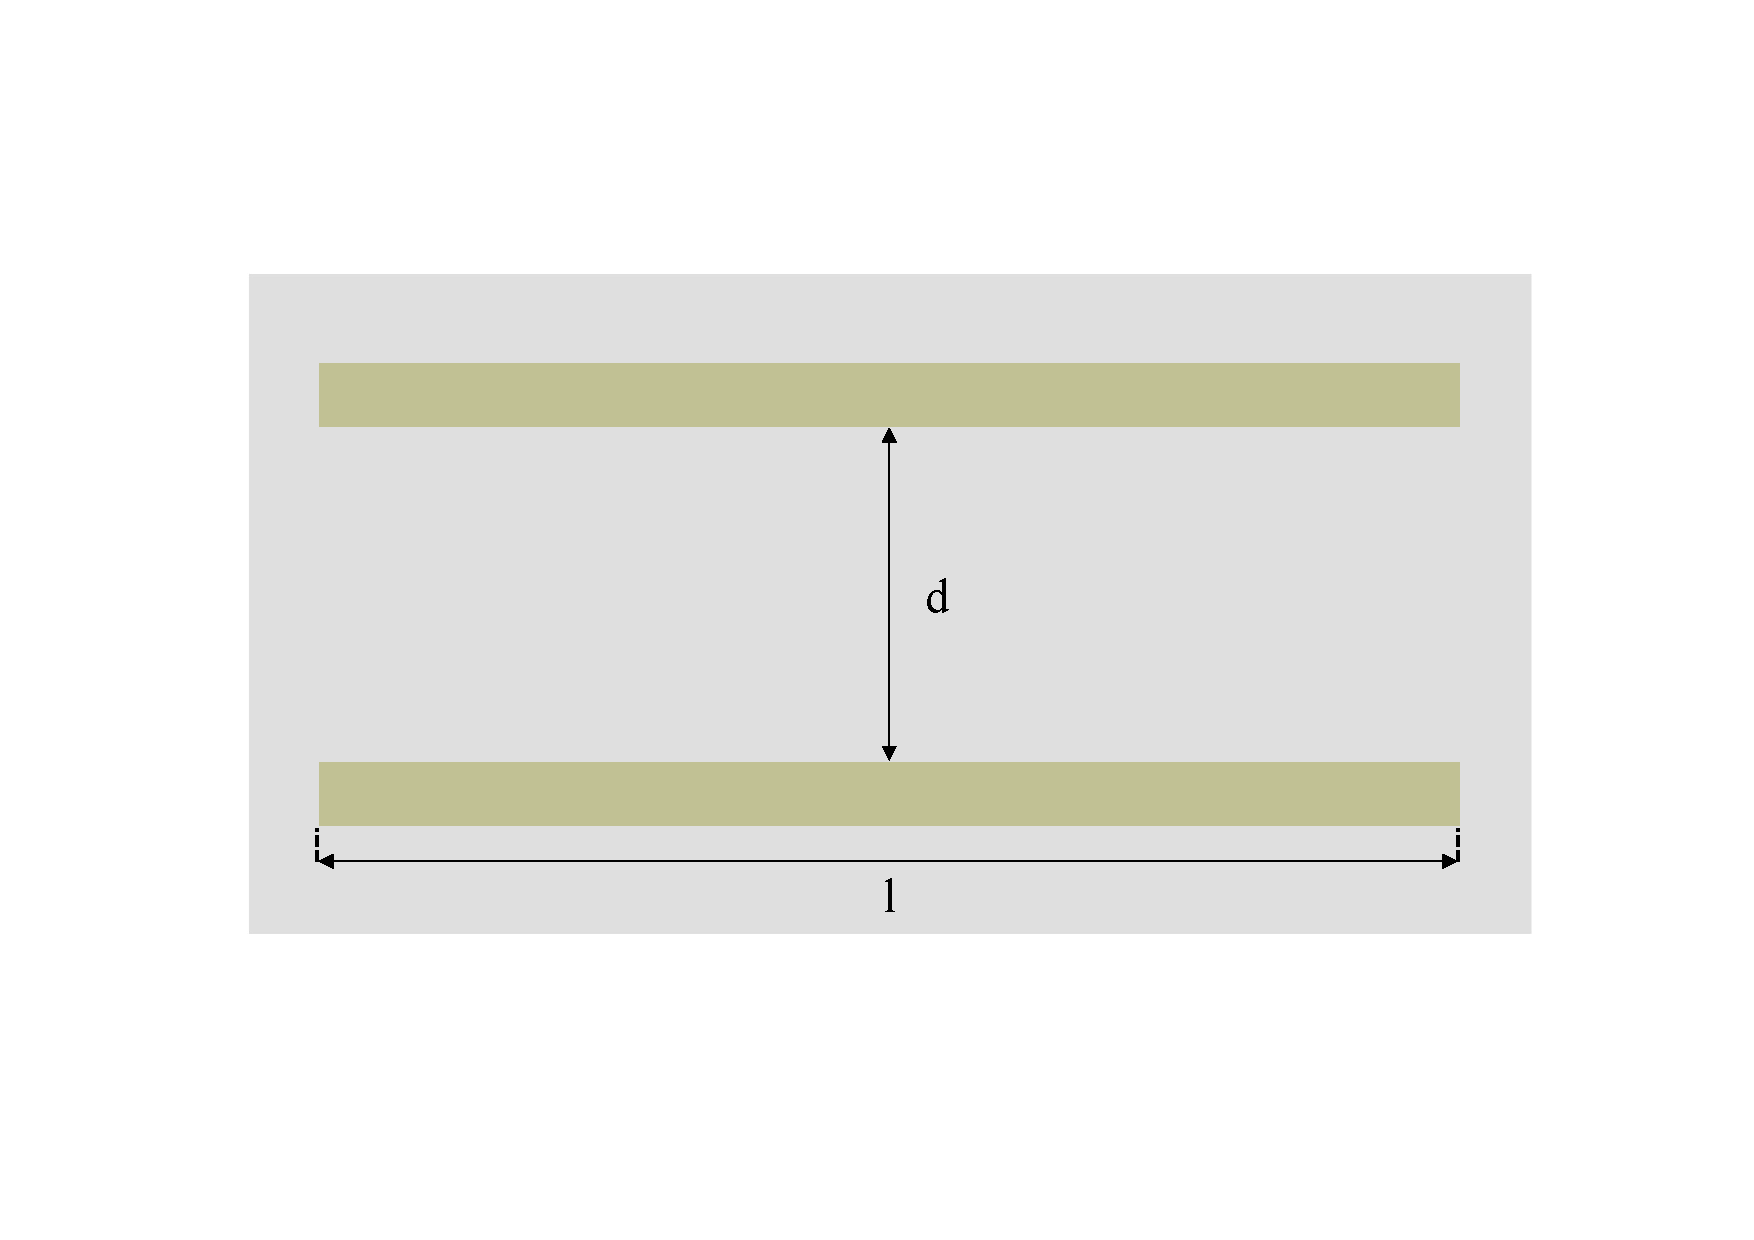
\includegraphics[width=8cm]{相互.pdf}
    \caption{2線路間に於ける相互インダクタンス}
\end{figure}
線路間の相互インダクタンスは配置によって以下の4通りのケースが存在する。
\begin{figure}[H]
    \centering
    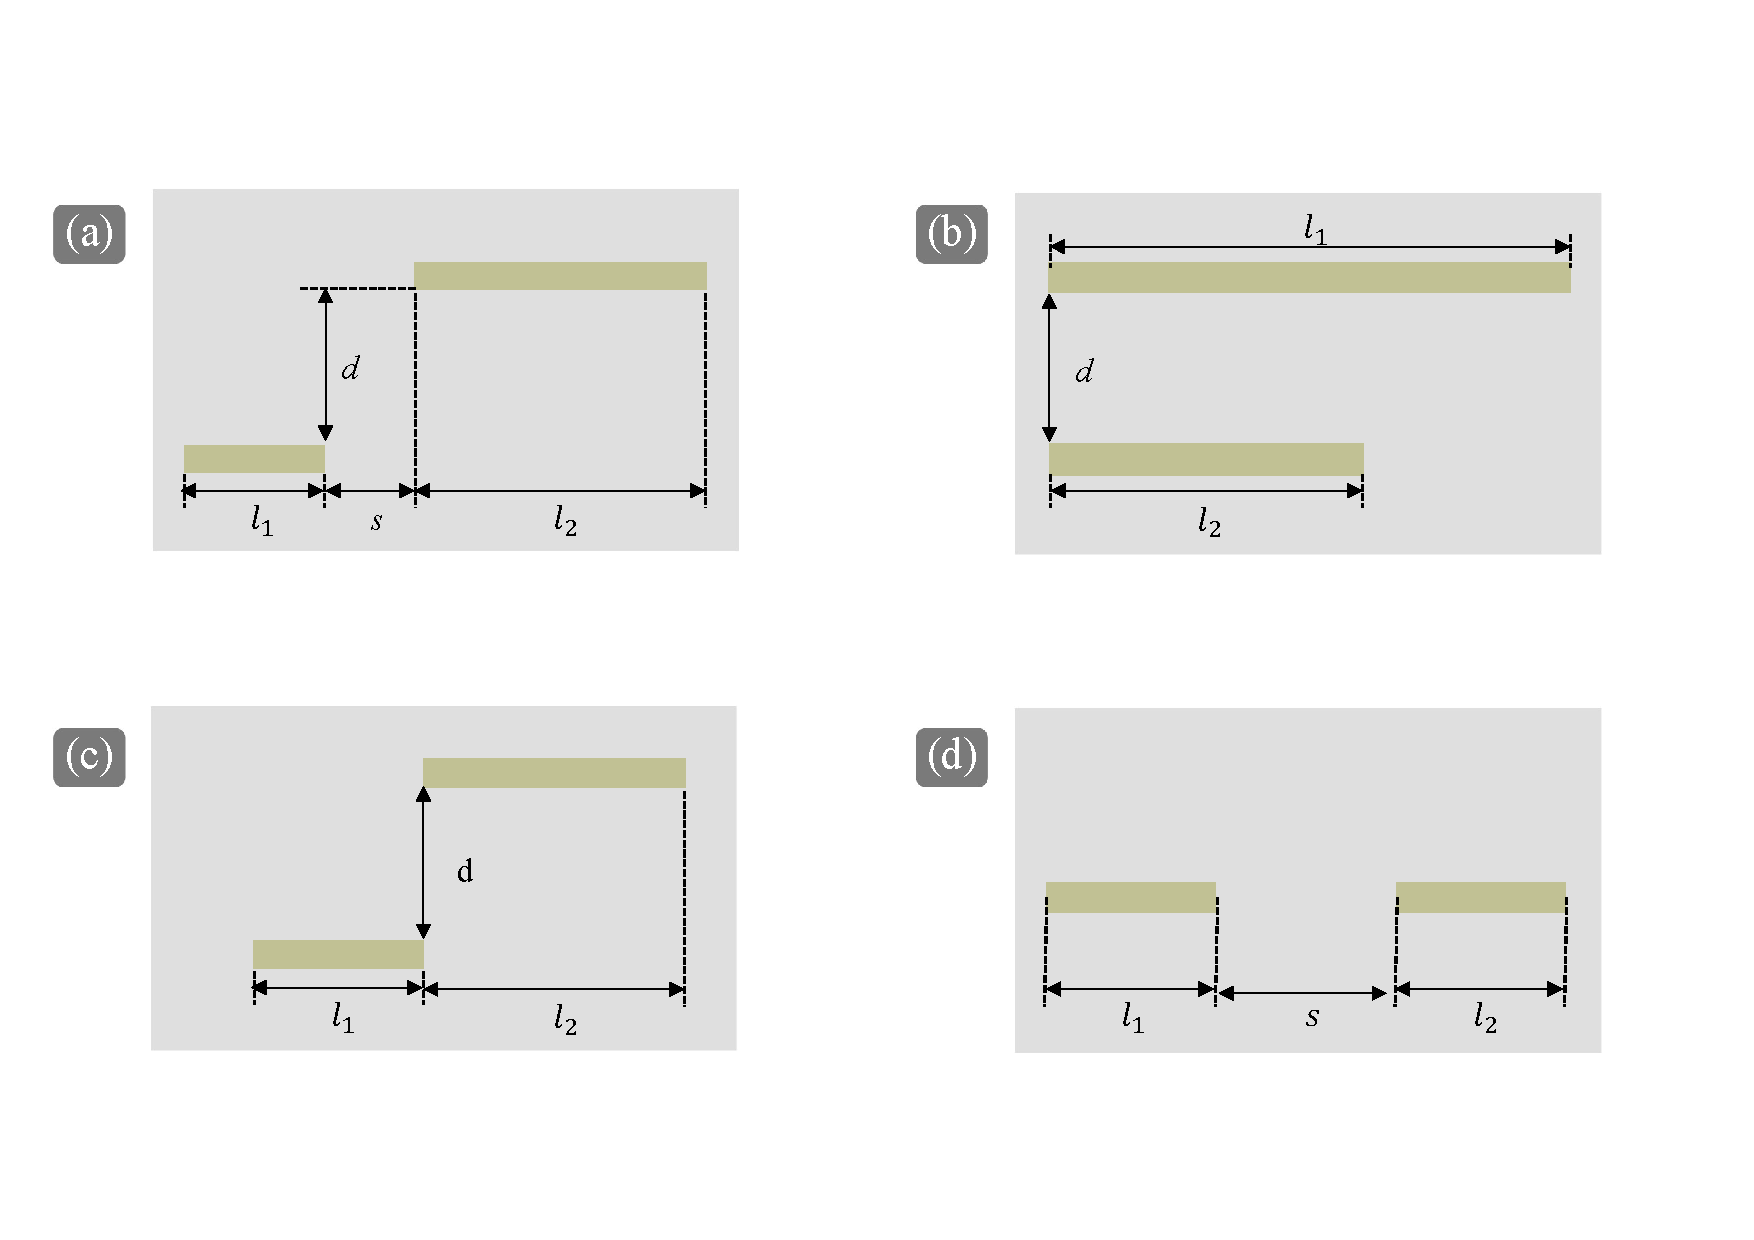
\includegraphics[width=14cm]{mutual.pdf}
    \caption{2線路間に於ける相互インダクタンス}
\end{figure}
よってそれぞれについて相互インダクタンスの関数を以下のように定義する。
\begin{equation}
    M_{a 1}\biggl(l_{1}, l_{2}, r, s\biggr)=0.5 \cdot\biggl(M_{c}\biggl(l_{1}+l_{2}+s, r\biggr)+M_{c}(s, r)-M_{c}\biggl(l_{1}+s, r\biggr)-M_{c}\biggl(l_{2}+s, r\biggr)\biggr)
\end{equation}
\begin{equation}
    M_{a 2}\biggl(l_{1}, l_{2}, r\biggr)=0.5 \cdot\biggl(M_{c}\biggl(l_{1}, r\biggr)+M_{c}\biggl(l_{2}, r\biggr)-M_{c}\biggl(l_{1}-l_{2}, r\biggr)\biggr)
\end{equation}
\begin{equation}
    M_{a 3}\biggl(l_{1}, l_{2}, r\biggr)=0.5\biggl(M_{c}\biggl(l_{1}+l_{2}, r\biggr)-M_{c}\biggl(l_{1}, r\biggr)-M_{c}\biggl(l_{2}, r\biggr)\biggr)
\end{equation}
\begin{equation}
    M_{b}\biggl(l_{1}, l_{2}, s\biggr)=\frac{\infty_{0}}{4 \pi}\biggl(\biggl(l_{1}+l_{2}+s\biggr) \ln \biggl(l_{1}+l_{2}+s\biggr)-\biggl(l_{1}+s\biggr) \ln \biggl(l_{1}+s\biggr)-\biggl(l_{2}+s\biggr) \ln \biggl(l_{2}+s\biggr)+s \ln (s)\biggr)
\end{equation}

上記の4通りの方法を各セグメントに適用することでミアンダインダクタンスに存在する相互インダクタンスをすべて勘定することができる。
偶奇それぞれについて計算する相互インダクタンスは以下の7ケースである。
\begin{figure}[H]
    \centering
    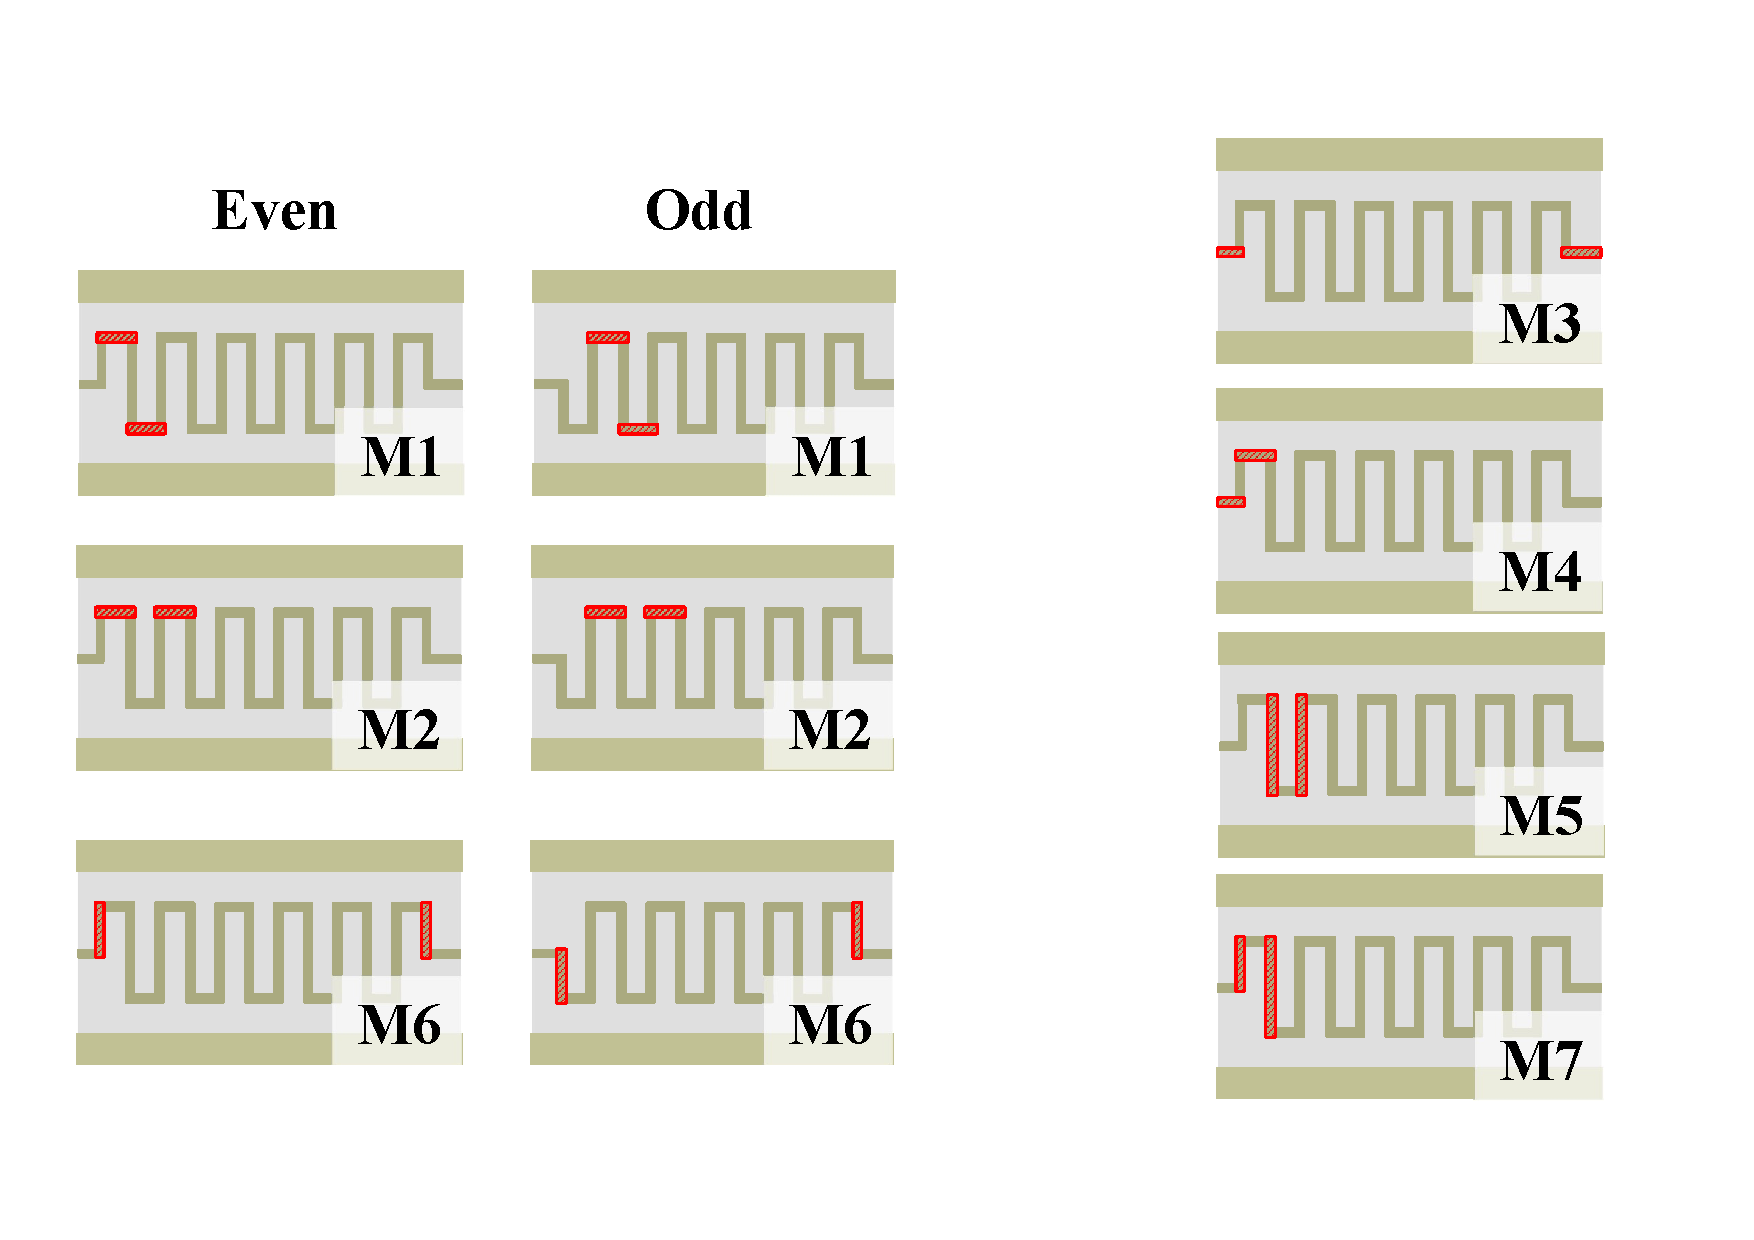
\includegraphics[width=14cm]{m2.pdf}
    \caption{セグメント別相互インダクタンス}
\end{figure}
上記のセグメント別の相互インダクタンスについて偶奇について違いあるものは
\begin{equation}
    \begin{array}{l}
    M_{1}=\sum_{i=1}^{N / 2}(2 N+4-4 i) \cdot M_{\mathrm{ul}}(d, d, h,(2 i-2) d), \text { for } N \text { even } \\
    \qquad M_{1}=\sum_{i=1}^{d}(2 N+4-4 i) \cdot M_{a 1}(d, d, h,(2 i-2) d), \text { for } N \text { odd }
    \end{array}
\end{equation}
\begin{equation}
    \begin{aligned}
    M_{2} &=\sum_{i=1}^{N / 2}(2 N+2-4 i) \cdot M_{b}(d, d,(2 i-1) d), \text { for } N \text { even } \\
    M_{2}=&\sum_{(N-1) / 2}^{\infty}(2 N+2-4 i) \cdot M_{b}(d, d,(2 i-1) d), \text { for } N \text { odd }
    \end{aligned}
\end{equation}
\begin{equation}
    \begin{aligned}
    M_{6}&=-2 \cdot M_{c}(b,(N+1) d), \text { for } N \text { even }\\
    M_{6}&=+2 \cdot M_{a 3}(b, b,(N+1) d), \text { for } N \text { odd }
    \end{aligned}
\end{equation}
また、偶奇の違いがないものについて
\begin{equation}
    M_{3}=2 \cdot M_{b}(a, a,(N+1) d)
\end{equation}
\begin{equation}
    M_{4}=\sum_{i=0}^{N} 4 \cdot M_{a 1}(a, d, b, i d)
\end{equation}
\begin{equation}
    M_{5}=\sum_{i=0}^{N-1}(-1)^{i} \cdot 2 \cdot(N-1) \cdot M_{c}(h, t d)
\end{equation}
\begin{equation}
    M_{7}=\sum_{i=0}^{N}(-1)^{i} \cdot 4 \cdot M_{a 2}\biggl(b_{2} h, i d\biggr)
\end{equation}
となる。それぞれについて各セグメントの総和
\begin{equation}
    M_{\text {tot }}=M_{1}+M_{2}+M_{3}+M_{4}+M_{5}+M_{6}+M_{7}
\end{equation}
によってミアンダインダクタンスに於ける相互インダクタンスを見積もることができる。これについて自己インダクタンスを足し合わせたもの
\begin{equation}
    L_{\text {tot }}=L_{\text {selftot }}+M_{\text {tot }}
\end{equation}
がミアンダインダクタンスとなる。ただし、本稿では線路として極低温下にある超伝導微細薄膜を用いているため線路長分のカイネティックインダクタンスを考慮する必要がある。


\section{マスター方程式}
\section{2点相関関数}
\section{等価回路}
本文中で電気回路に於ける基本的な回路の等価変換を行った。ここでは、2端子対回路に於ける等価回路について解説する。\cite*{電気回路,続電気回路の基礎}
電気回路を考える場合入力と出力を考え、上図のように定めると都合がよい。この回路網が満たす条件をここでは
①内部に電源を含まない。ただし、トランジスタの直流電源は差し支えない。
②線形であっても重ね合わせの原理が成立する。
③入力埜1端子から流れ込んだ電流は入力の他端子から流れ出る。出力側も同様である。
2端子対回路は幾通りかの特性表示の方法があり、ここではFパラメータを用いる。Fパラメータを用いる場合の2端子対回路の電流電圧は上図のように表現される。
\begin{figure}[H]
    \centering
    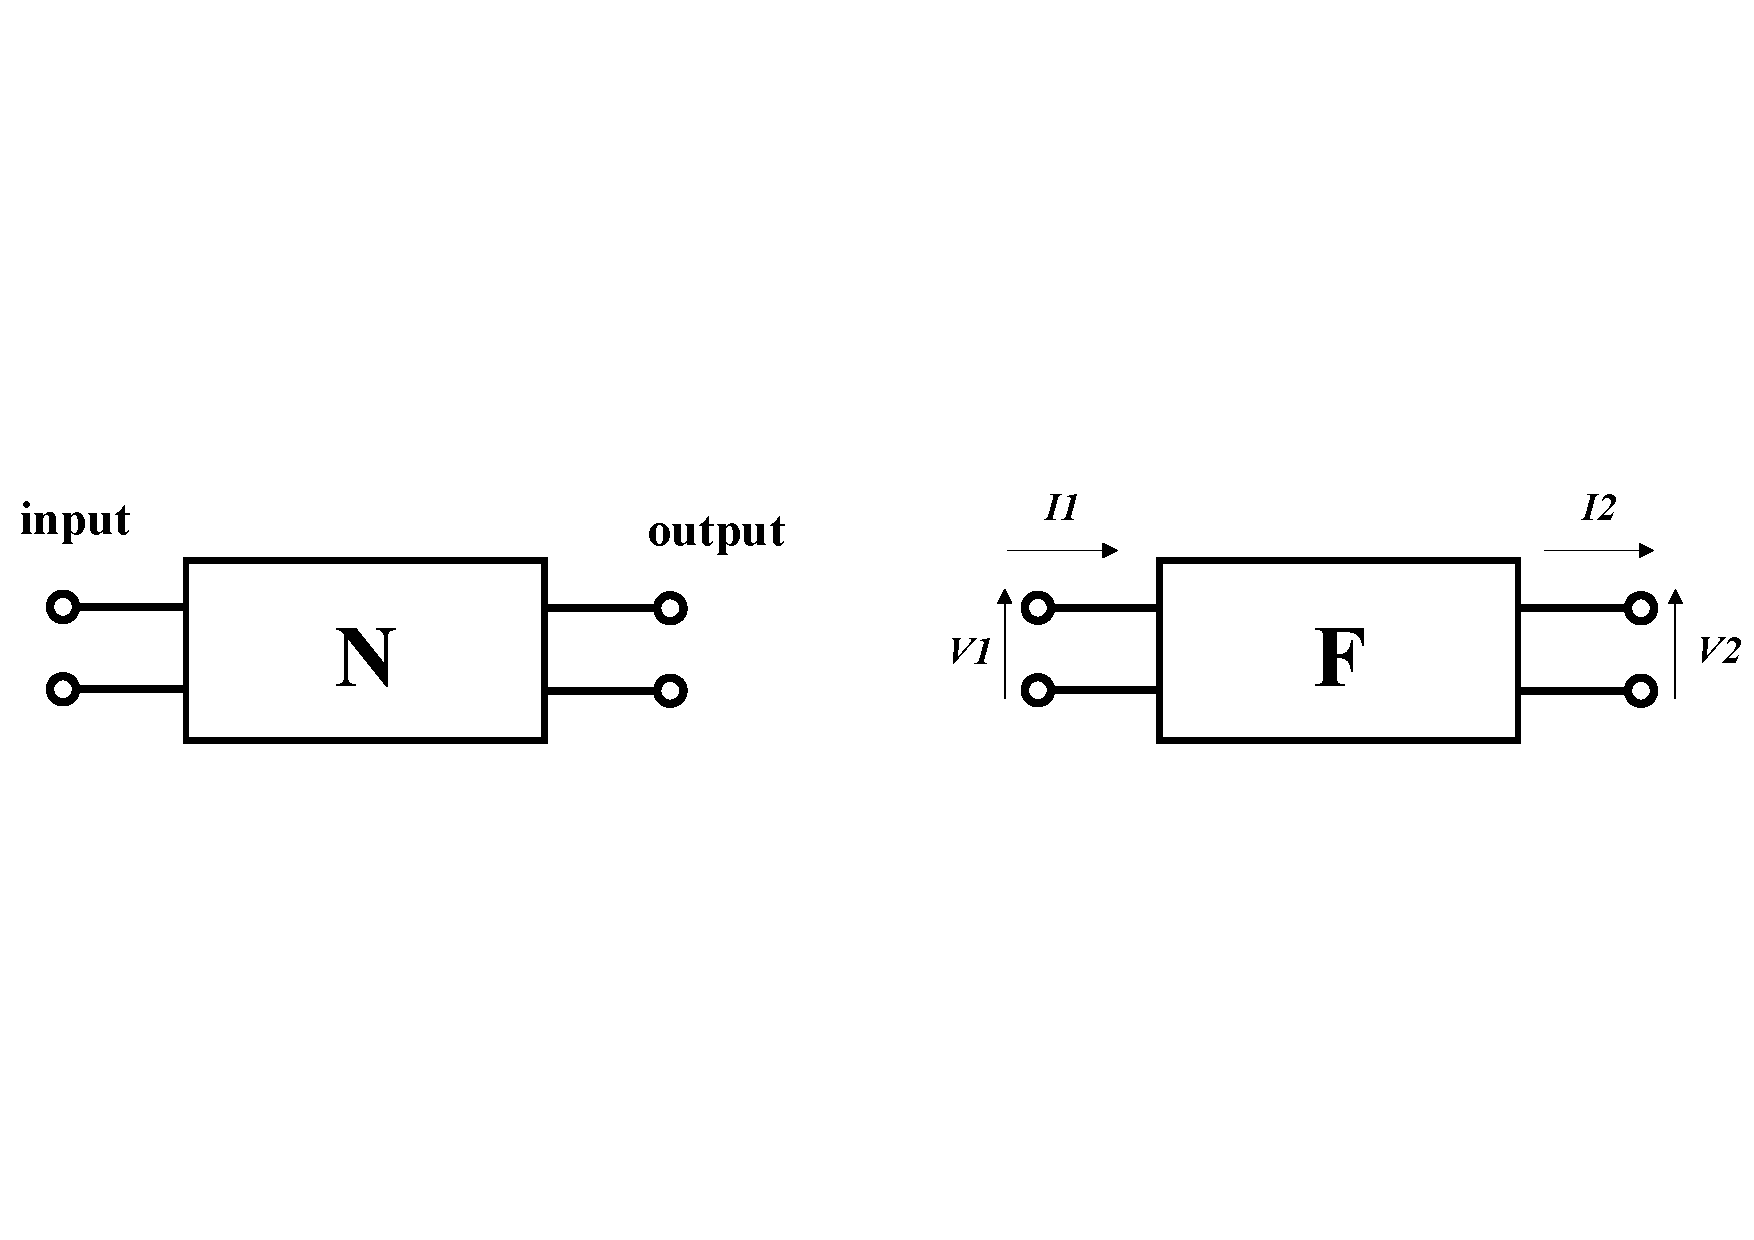
\includegraphics[width=8cm]{2端子.pdf}
    \caption{2端子対マトリックス}
\end{figure}
この場合Fマトリックスは次式で与えられる。
\begin{eqnarray}
    V_1 &= AV_2 + BI_2\\
    I_1 &= CV_2 +DI_2 
\end{eqnarray}
\begin{equation*}
    \begin{pmatrix}V_1\\I_1\end{pmatrix} = \begin{pmatrix}A&B\\C&D\end{pmatrix}\begin{pmatrix}V_2\\I_2\end{pmatrix}
\end{equation*}
\begin{equation*}
    F = \begin{pmatrix}A&B\\C&D\end{pmatrix}
\end{equation*}
この時、行列要素A,B,C,Dについてそれぞれの次元はA(無次元),B($\Omega$),C(S),D(無次元)である。次元Sは伝導度であり、$\Omega$の逆数である。
Fパラメータを用いる理由は複数の2端子回路を組み合わせた時に計算が簡便になるためである。ここで、2端子回路の接続について考える。
\begin{equation*}
    \begin{pmatrix}V_1\\I_1\end{pmatrix} = \begin{pmatrix}A1&B1\\C1&D1\end{pmatrix}\begin{pmatrix}V_2\\I_2\end{pmatrix}
\end{equation*}
\begin{equation*}
    \begin{pmatrix}V_2\\I_2\end{pmatrix} = \begin{pmatrix}A2&B2\\C2&D2\end{pmatrix}\begin{pmatrix}V_3\\I_3\end{pmatrix}
\end{equation*}
したがって
\begin{equation*}
    \begin{pmatrix}V_1\\I_1\end{pmatrix} = \begin{pmatrix}A1&B1\\C1&D1\end{pmatrix}\begin{pmatrix}A2&B2\\C2&D2\end{pmatrix}\begin{pmatrix}V_3\\I_3\end{pmatrix}
\end{equation*}
\begin{equation*}
    \begin{pmatrix}V_1\\I_1\end{pmatrix} = F1 F2 \begin{pmatrix}V_3\\I_3\end{pmatrix}
\end{equation*}
\begin{equation*}
    \begin{pmatrix}V_1\\I_1\end{pmatrix} = F \begin{pmatrix}V_3\\I_3\end{pmatrix}
\end{equation*}
すなわちFパラメータ表現では、各回路の接続は行列の積として与えられる。
この性質を用いてFパラメータを用いて2通りの2端子対回路を示す。
\subsection{T型回路}
図のようにインピーダンス素子を配置したときFパラメータを用いてどのように表現されるかを示す。
\begin{figure}[H]
    \centering
    \includegraphics[width=10cm]{t型.pdf}
    \caption{T型2端子回路}
\end{figure}
Fパラメータの積の性質及び、各行列要素に適切な値を入力することでT型回路のFパラメータは
\begin{eqnarray}
    \begin{pmatrix}A&B\\C&D\end{pmatrix} &= \begin{pmatrix}1&Z1\\0&1\end{pmatrix}\begin{pmatrix}1&0\\\frac{1}{Z2}&0\end{pmatrix}\begin{pmatrix}1&Z3\\0&1\end{pmatrix}\\
    &=\begin{pmatrix}1+\frac{Z1}{Z2}&Z1+Z3+\frac{Z1Z3}{Z2}\\\frac{1}{Z2}&1+\frac{Z3}{Z2}\end{pmatrix}
\end{eqnarray}
\subsection{$\Pi$型回路}
同様にして$\Pi$型回路についてFパラメータを求めると
\begin{figure}[H]
    \centering
    \includegraphics[width=10cm]{pi型.pdf}
    \caption{$\Pi$型2端子回路}
\end{figure}
\begin{eqnarray}
    \begin{pmatrix}A&B\\C&D\end{pmatrix} &= \begin{pmatrix}1&Z1\\0&1\end{pmatrix}\begin{pmatrix}1&0\\\frac{1}{Z2}&0\end{pmatrix}\begin{pmatrix}1&Z3\\0&1\end{pmatrix}\\
    &=\begin{pmatrix}1+\frac{Z1}{Z2}&Z1+Z3+\frac{Z1Z3}{Z2}\\\frac{1}{Z2}&1+\frac{Z3}{Z2}\end{pmatrix}
\end{eqnarray}
\subsection{$T-\Pi$変換($Y-\Delta$変換)}
以上の2つの回路についてそれぞれのFパラメータを比較することで回路の等価変換を行うことができる。便宜状T型のインピーダンスをZ、$\Pi$型のインピーダンスをXとして表すと
\\
$\Pi$型\\
\begin{eqnarray}
    \begin{pmatrix}A&B\\C&D\end{pmatrix} &= \begin{pmatrix}1&X1\\0&1\end{pmatrix}\begin{pmatrix}1&0\\\frac{1}{X2}&0\end{pmatrix}\begin{pmatrix}1&X3\\0&1\end{pmatrix}\\
    &=\begin{pmatrix}1+\frac{X1}{X2}&X1+X3+\frac{X1X3}{X2}\\\frac{1}{X2}&1+\frac{X3}{X2}\end{pmatrix}
\end{eqnarray}
T型\\
\begin{eqnarray}
    \begin{pmatrix}A&B\\C&D\end{pmatrix} &= \begin{pmatrix}1&Z1\\0&1\end{pmatrix}\begin{pmatrix}1&0\\\frac{1}{Z2}&0\end{pmatrix}\begin{pmatrix}1&Z3\\0&1\end{pmatrix}\\
    &=\begin{pmatrix}1+\frac{Z1}{Z2}&Z1+Z3+\frac{Z1Z3}{Z2}\\\frac{1}{Z2}&1+\frac{Z3}{Z2}\end{pmatrix}
\end{eqnarray}

連立方程式を解くとそれぞれ
\begin{eqnarray}
    X1 &= \frac{Z1Z2+Z2Z3+Z3Z1}{Z3}\\
    X2 &= \frac{Z1Z2+Z2Z3+Z3Z1}{Z2}\\
    X3 &= \frac{Z1Z2+Z2Z3+Z3Z1}{Z1}\\
\end{eqnarray}
また、この逆は
\begin{eqnarray}
    Z1 &= \frac{X1X2}{X1+X2+X3}\\
    Z2 &= \frac{X3X1}{X1+X2+X3}\\
    Z3 &= \frac{X2X3}{X1+X2+X3}\\
\end{eqnarray}
となる。
次にインダクタンスにより磁気的に結合された回路をT型回路によって表示する方法を以下に示す。
\subsection{磁気結合回路}
磁気的に結合された回路を以下のように表す。この回路表記は変圧器の回路表現と同等である。
\begin{figure}[H]
    \centering
    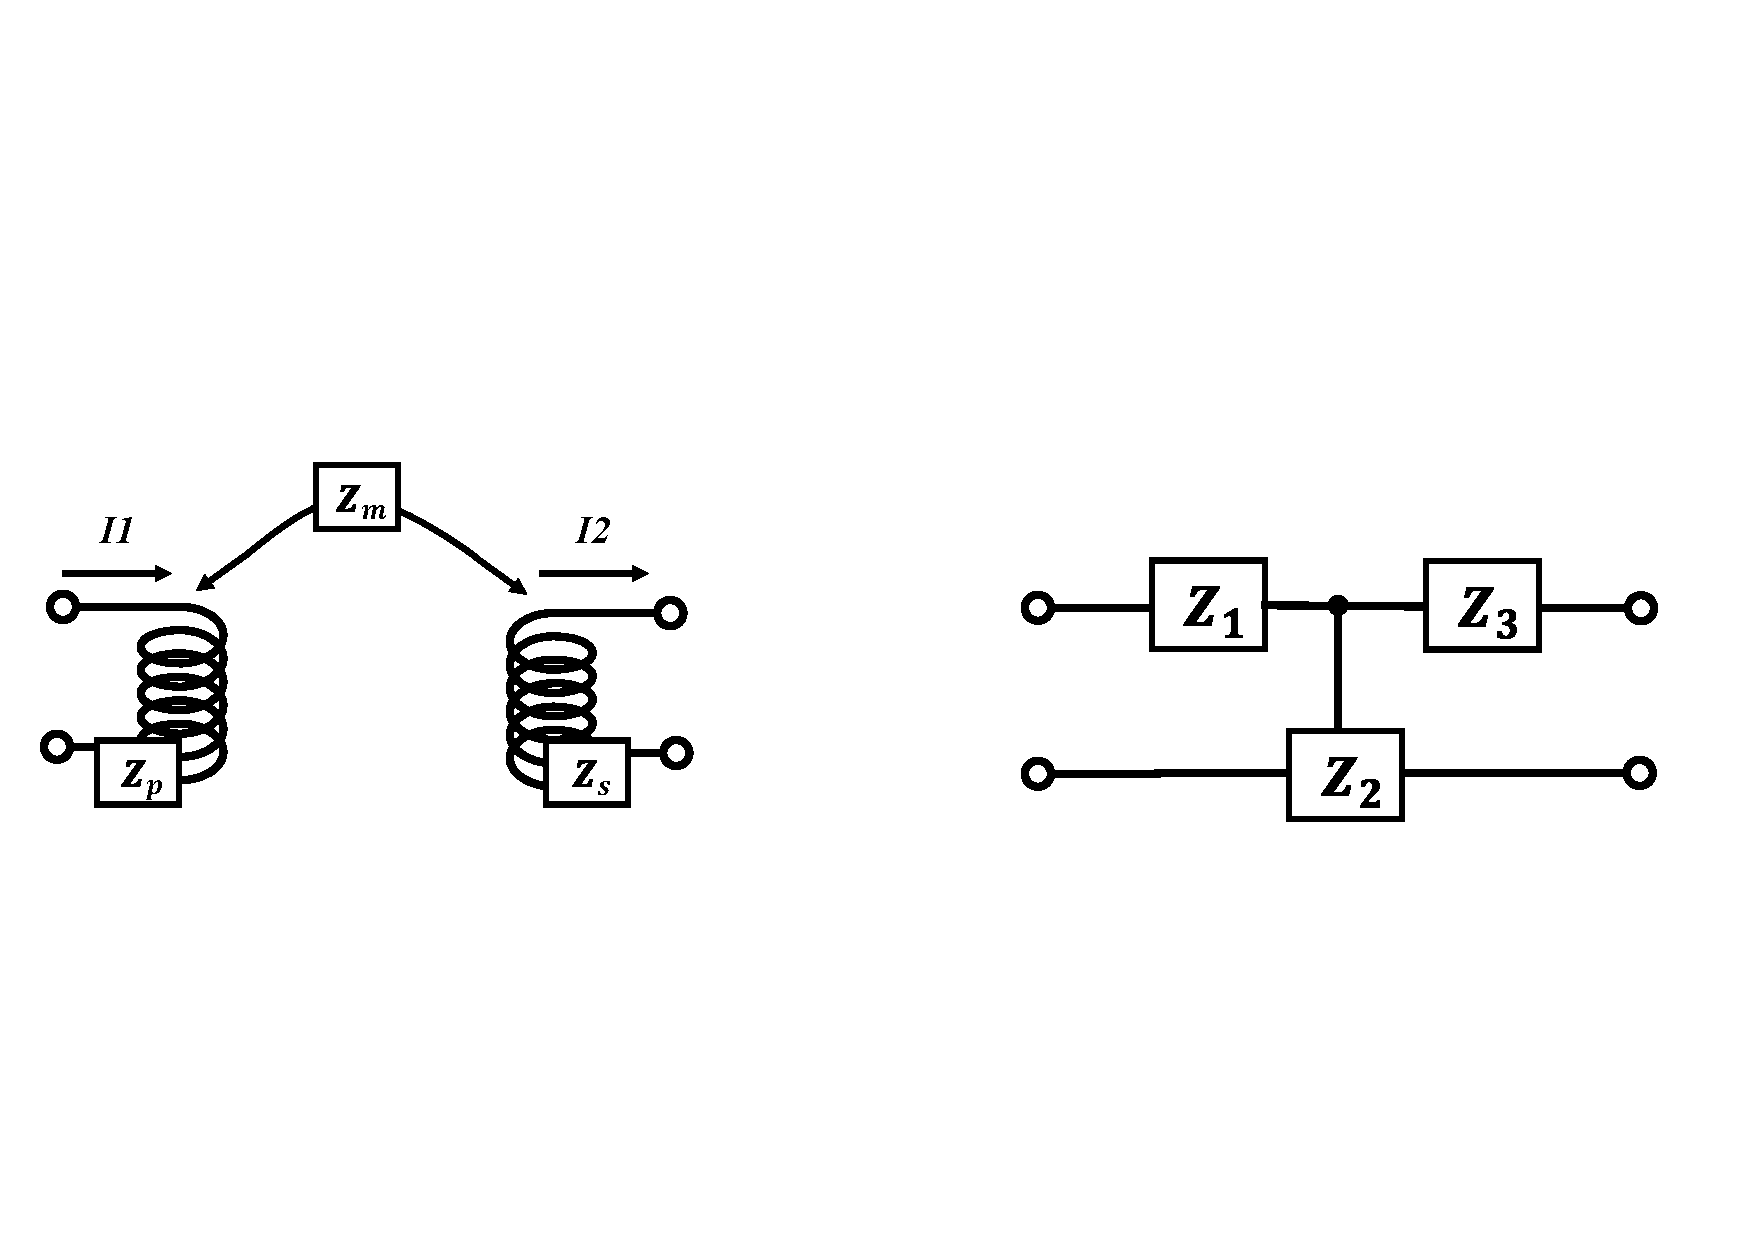
\includegraphics[width=12cm]{磁気的結合回路.pdf}
    \caption{磁気的結合回路}
\end{figure}
Zmは通常相互インダクタンスMを用いて
\begin{equation*}
    Z_m = \pm i\omega M
\end{equation*}
として表現できる。
変圧器のFパラメータを求めるためにキルヒホッフの法則より電圧と電流の関係は
\begin{eqnarray}
    V_1 &= Z_p I_1 -Z_m I_2\\
    -V_2 &= -Z_m I_1 + Z_s I_2\\
\end{eqnarray}
上式を整理して
\begin{eqnarray}
    V_1 &= \frac{Z_P}{Z_M}V_2 - \frac{Z_PZ_S-Z_M^2}{Z_M}I2\\
    I_1 &= \frac{1}{Z_M}V_2+\frac{Z_S}{Z_M}I_2
\end{eqnarray}
行列表現に直すことでFパラメータが
\begin{equation*}
    \begin{pmatrix}A&B\\C&D\end{pmatrix} =\begin{pmatrix}1+\frac{Z_P}{Z_M}&\frac{Z_PZ_S-Z_M^2}{Z_M}\\\frac{1}{Z_M}&1+\frac{Z_S}{Z_M}\end{pmatrix}
\end{equation*}
と求まる。T型と比較すると
\begin{eqnarray}
    Z_1 &= Z_P-Z_M\\
    Z_2 &= Z_M\\
    Z_3 &= Z_S-Z_M
\end{eqnarray}
と表現することができる。インダクタンスLを用いてよりあらわに以上の関係を図式すると
\begin{figure}[H]
    \centering
    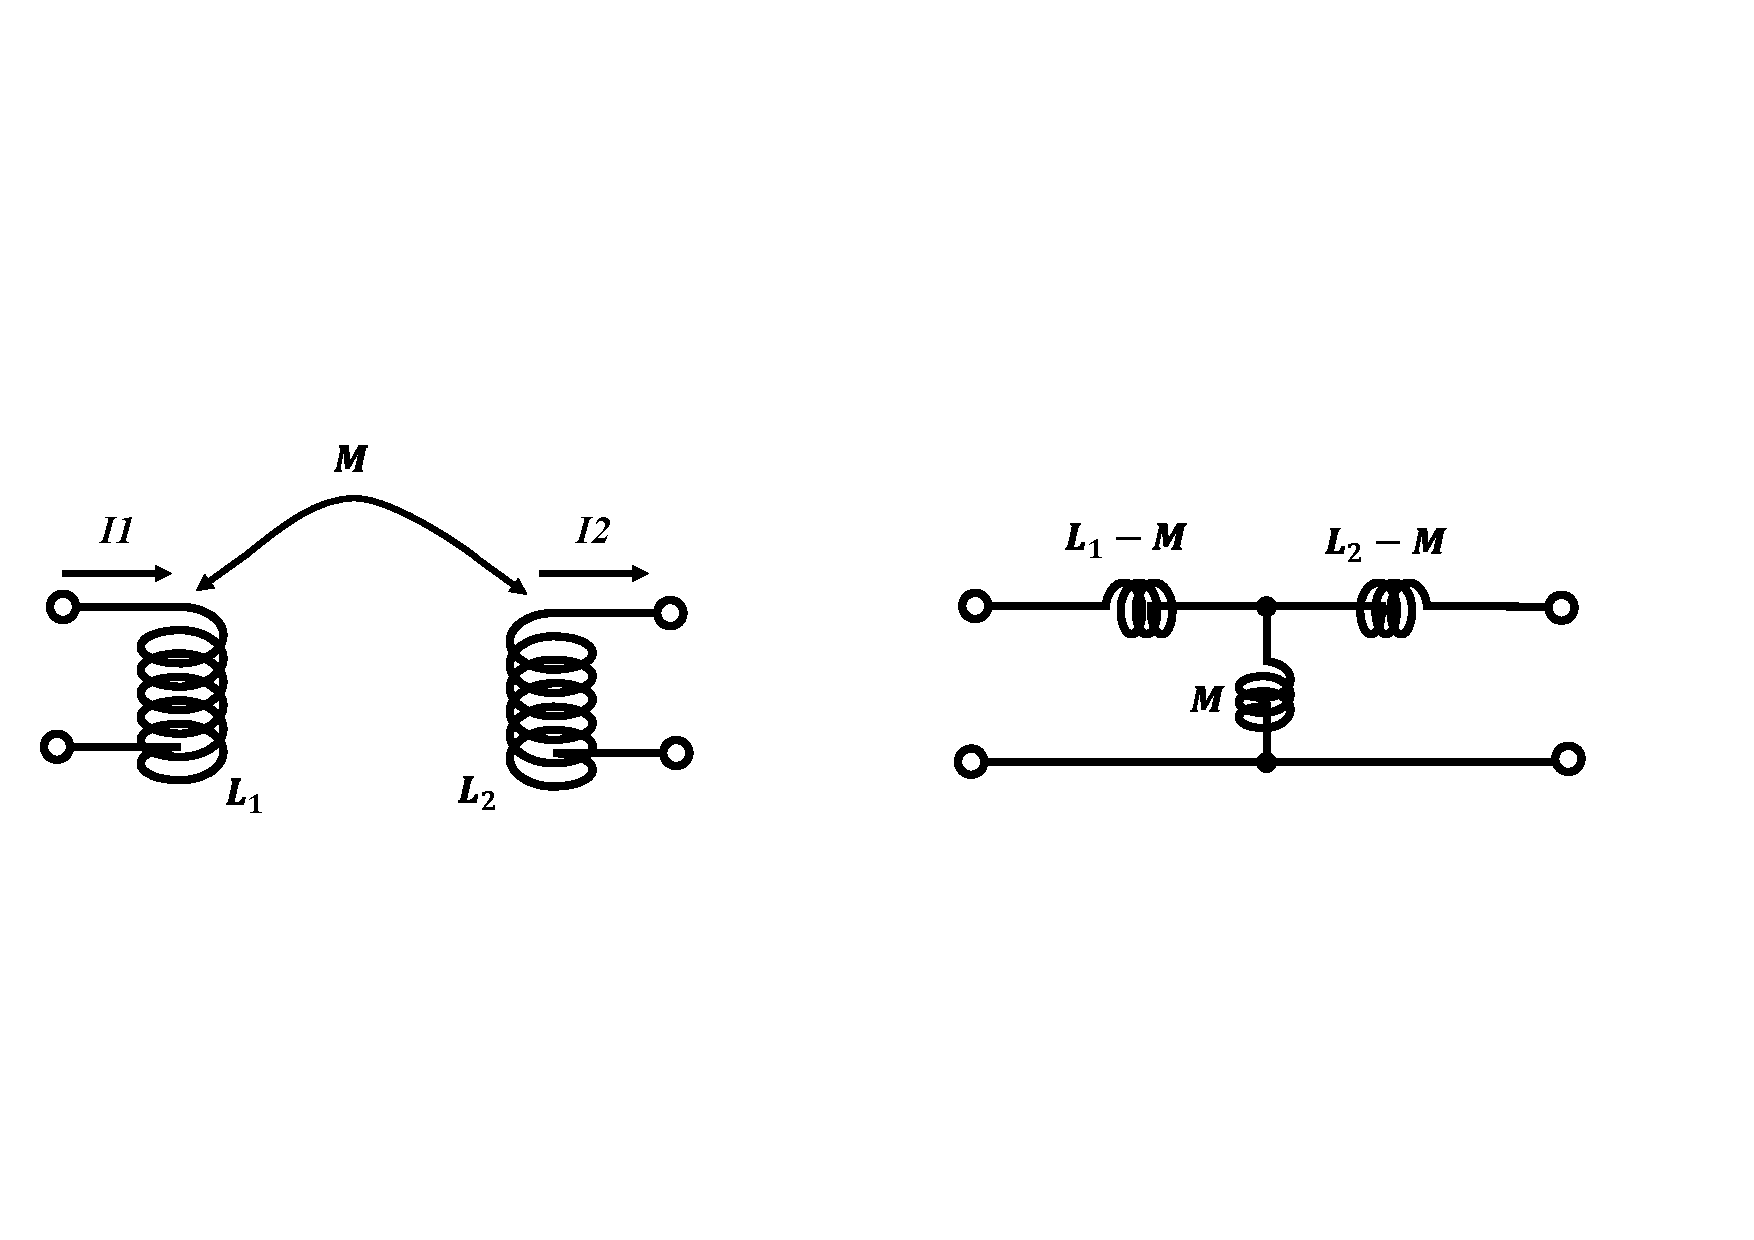
\includegraphics[width=12cm]{変圧器.pdf}
    \caption{変圧器とT型回路}
\end{figure}
